\documentclass[index]{subfiles}

\begin{document}
\title{Noise Cancellation}
\author{by Shengdong Li}
\date{26 October 2021}
\maketitle

\section{Research Question}

How does the difference in phase between two waves affect the sound level at a certain point between them?

\section{Background}

My home has always been slightly noisy, perhaps due to its positioning facing the living room, or perhaps due to my little brother's whining. I've tried blocking the door with a mattress, or blocking my own ears with some headphones, but I've never thought of blocking a sound wave with another sound wave until hearing of the concept of wave interference of light in my phyiscs class. I do have a set of speakers, connected to my computer. This lab aims to explore both the mechanics and concepts behind noise-cancellation, as well as explore at what delays between phases is noise-cancellation the most optimal.

\subsection{Wave Interference}

The waves explored in this lab both have the same frequency and wavelength, so the first thing that comes to mind between these two waves that might cause a change in sound intensity is wave interference.
Wave interference essentially occurs, when two waves meet together. There are two types of wave interference: constructive and destructive interference, which occur depending on the relative position of the two waves. When identical waves match up exactly, perfect constructive interference may occur, causing the amplitude of the resulting wave to double. Conversely, when the two waves are exactly \(\frac{1}{2}\lambda\) apart in position, they are out of phase, and perfect destructive interference occurs, which causes the effective amplitude of the resulting combined wave to be zero. \cite{openstax}

\subsection{Sound Intensity}

We know from theory that the relative phase shift between two waves is clearly tied to amplitude of the resulting wave in some way, but the amplitude doesn't necessarily equal the sound level of the wave. In fact, the energy of the wave is proportional to the square of its amplitude \cite{openstax}. This is because kinetic energy is equivalent to \(\frac{1}{2}mv^{2}\), and when the amplitude of the wave increases the effective velocity increases (?) \cite{openstax}.

The sound intensity of a wave depends both on the energy of the wave and the area in which it travels through, being proportional to power and inversely proportional to area as shown by \(I=\frac{P}{A}\), where area is a square length. \cite{openstax}.

\subsection{Sound Level}

However, while sound intensity is useful for calculating energy levels, humans don't react to sound intensity at a linear level. Instead, it's more of an exponential relationship. Decibels factor this in, as louder sounds need exponentially more energy in order to sound "louder" to humans.

This equation can be given by
$$
    \beta\left(dB\right)=10\log_{10}\left(\frac{I}{I_{0}}\right)
$$, where \(I_{0}\) is a constant \cite{openstax}.

The average sound level of a normal conversation around 70 decibels.\cite{speakers}.

\subsection{Speakers}

Because the sound waves of this experiment will be generated by speakers, it is necessary to understand, at least at a basic level, how speakers function. \cite{speakers}

For dynamic speakers, sound is generated from electric signals. When electric signals travel into a coil, a magnetic field is generated, and this causes an oscillatory motion between the cone and the coil \cite{openstax} \cite{speakers}, resulting in motion and therefore sound waves to be produced.

\section{Hypothesis}

The difference in displacement between two in-phase waves would have a sinusoidal relationship with the sound intensity level, due to constructive and destructive interference causing cyclic patterns of change in amplitude of the resulting sound.

% \subsection{Prediction Graph (remove later)}


% \begin{figure}[H]
%     \centering
%     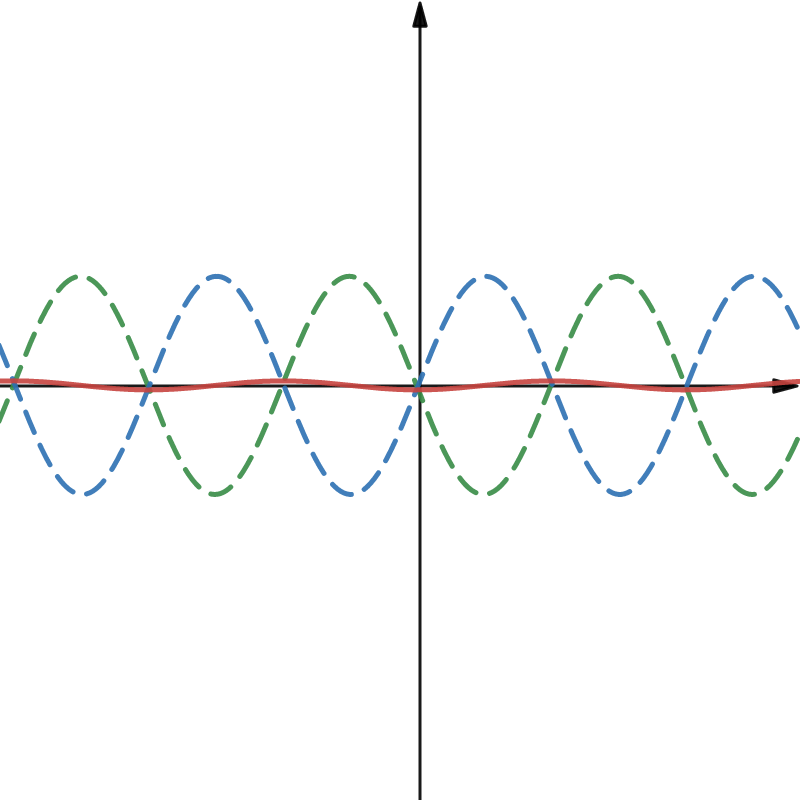
\includegraphics[scale=0.3]{prediction.png}
%     \caption{Predicted graph. Red line is the resulting amplitude. \href{https://www.desmos.com/calculator/ahmohu46il}{link}}
% \end{figure}

\section{Variables and Explanations}

\subsection{Independent Variable}

The independent variable in this case would be the phase-shifted distance between the two waves. Its units are in a decimal of the wavelength of a sine wav with a frequency of 250 Hz.

As the sounds from the speakers are generated by sampling a \(\sin\) function with a frequency of 250 Hz, this independent variable will be directly set by adding an it as an offset, \(\sin(x + dt)\), where \(\dt\) is the phase shift, to the second speaker on the right.

The uncertainty in this independent variable is practically negligible, as the increments in phase shift are directly set in the computer program as floating point values.

\subsection{Dependent Variable}

The sound level will be the dependent variable of the equation. It will be in the units of decibel. This measurement will be taken with the microphone on a used samsung galaxy sx running the recording app xxx, for ten seconds. Then samples will be taken every second and averaged. 

The uncertainty here will arise from the sensitivity of the microphone.

\subsection{Controlled Variable}

\textbf{The distance between the two speakers} must be kept constant in every trial. As sound spreads out, it loses power exponentially, so pulling the speakers too far apart would generally decrease the sound level, and pulling the speakers too close together would increase the sound level. The distance between the two speakers would also directly impact the independent variable, the phase shift between two waves. For example, for a \(\sin\) wave of 250 Hz (around middle C frequency), the wavelength is only \(1.3m\), so a small shift in speaker distance in the tens of centimeters could invalidate the whole experiment.

\textbf{The position of the microphone} should be kept constant in every trial. This is because while for perfect destructive interference the amplitude of the wave everywhere would be zero, because sound waves are sinusoidal their amplitudes differ at certain points. A distance further away from the source would also result in decreasing sound levels due to the fact that energy travels away in a sphere so much of it is lost to the environment further out.

\textbf{The frequency and wavelength of the two waves} The frequency of two waves should be kept the exact same throughout all trials. In order for perfect constructive and destructive interference to occur, the two waves must be perfectly in-phase with each other, otherwise the resulting wave would be very uneven and there would be varying results everytime.

\textbf{The temperature of the room} The temperature of the room should be kept constant because temperature and movement of particles in the air affects the amount of energy lost as the wave propogates forward.

\textbf{Ambient Sound Level} The ambient sound level should be kept constant because otherwise the dependent variable of sound level would be modified not just by the independent variable but also by the environment, which would invalidate the experiment. To minimize the impact that the environment will have on the experiment, four chairs will be placed surrounding the two speakers, and plankets draped over them and the top of the speakers, in an effort to decrease the effects that ambient sound levels would have on the final experiment.

\section{Method}

\begin{figure}[H]
    \centering
    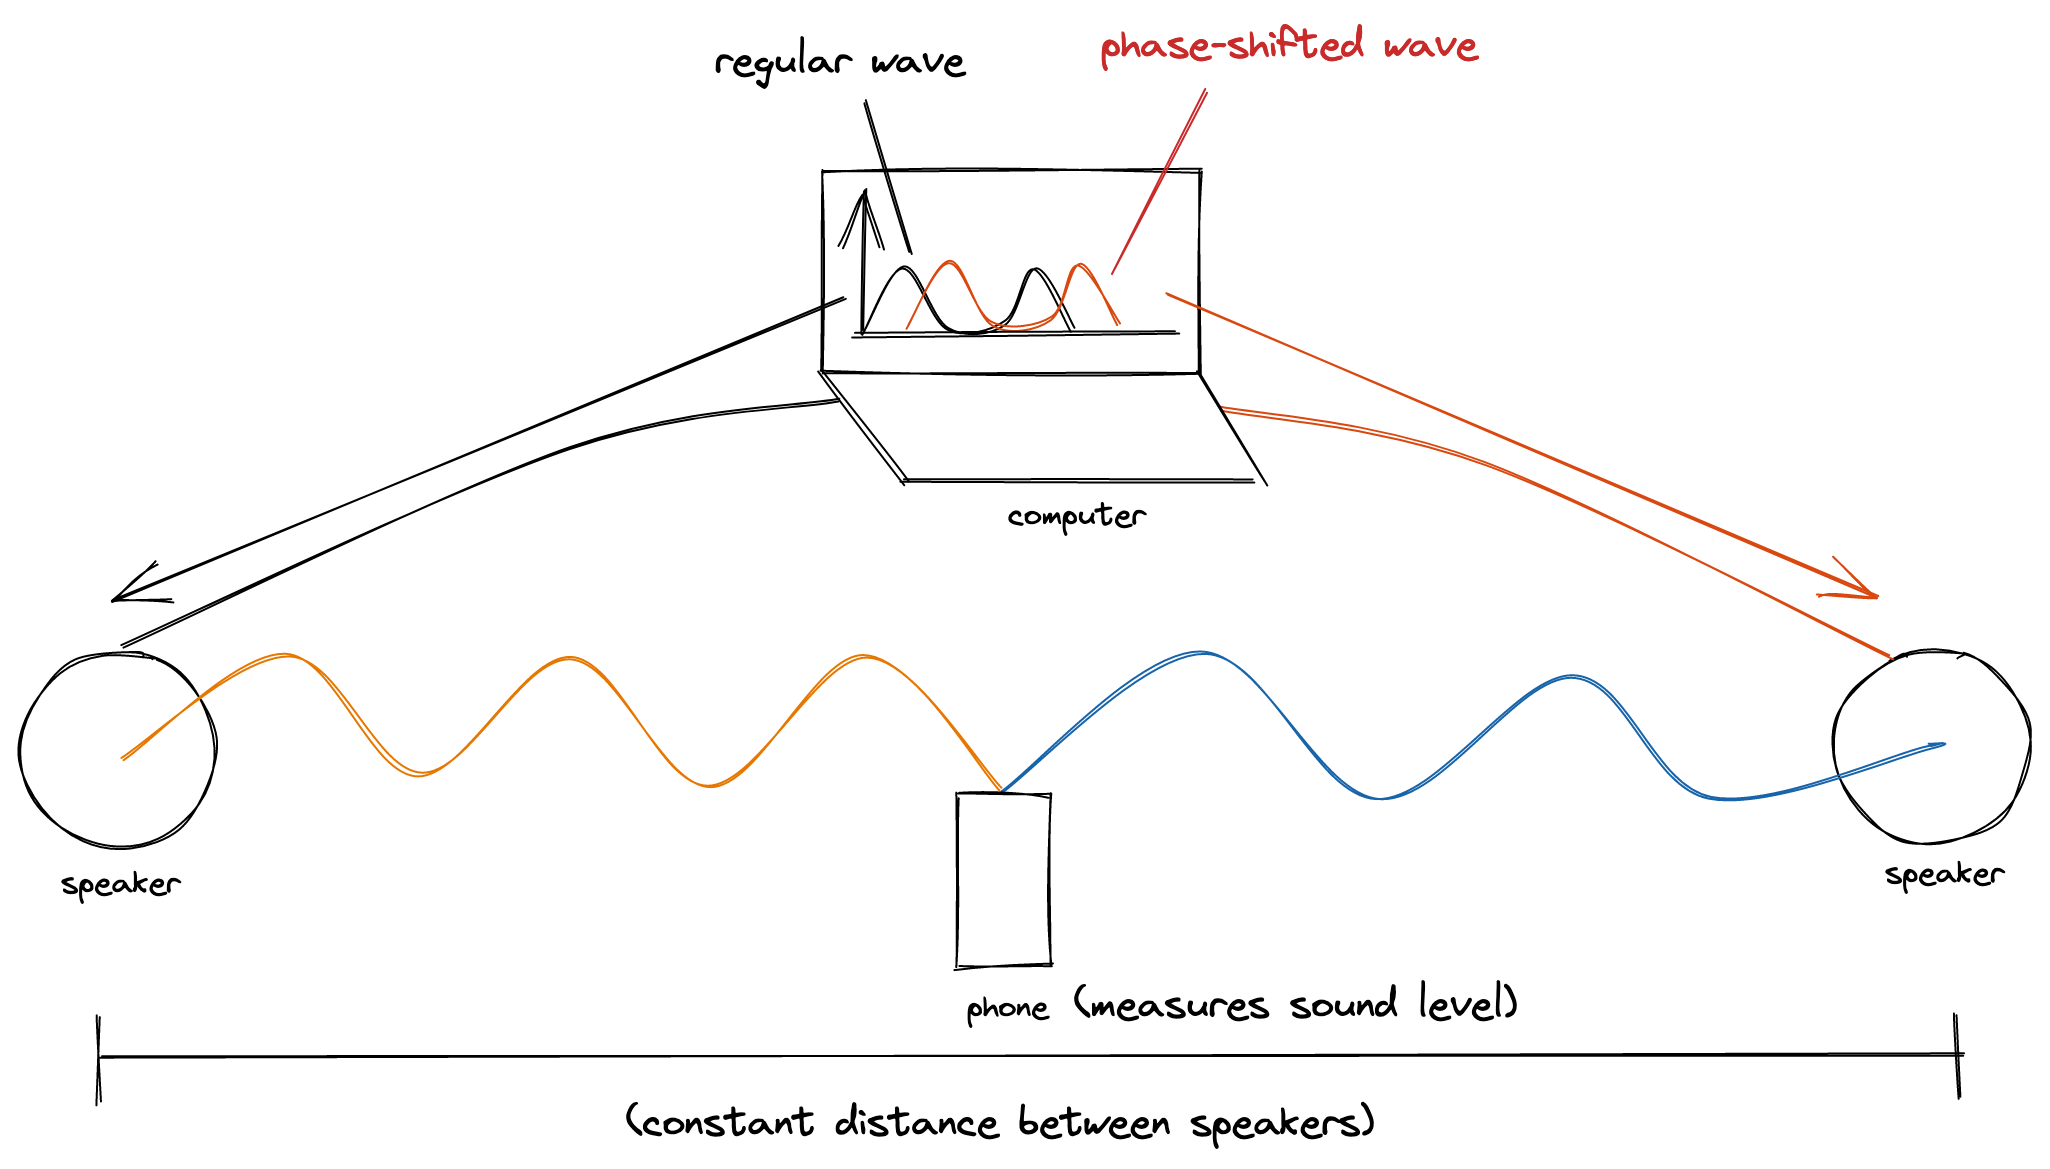
\includegraphics[scale=0.24]{sound_diagram.png}
    \caption{Sketch of experiment setup.}
\end{figure}

\begin{enumerate}
    \item Position two identical speakers 1.3 meters apart from each other, with their fronts facing directly towards each other
    \item Connect both speakers via cable to a computer
    \item Put a phone face up between the middle of the two speakers
    \item Run a computer program that plays a monotone sine wave at a frequency of 250 Hz through one speaker, then plays the exact same sound on the other speaker
    \item After the speakers have started playing for at least 5 seconds, begin recording audio on the phone for 20 seconds.
    \item After 20 seconds, pause, and record the average sound level displayed on the app
    \item Repeat this recording process 3 times, and take the average of the three trials
    \item Repeat the entire experiment with shifted wavelengths of 0, incrementing by \(0.05\times\lambda\), all the way up to and including a full phase shift of \(1\lambda\)
\end{enumerate}

\subsection{Safety}

Safety precautions should be made to ensure that the speaker sound levels do not go above maximal decibel sound levels that humans are tolerant of, to preserve the health of the ear.

\section{Evaluation and Discussion}???

\subsection{Strengths}

The use of a computer to change the independent variable, change in phase between two identical waves, offers a very high degree of accuracy, especially in dealing with waves travelling at the speed of light. This should result in a very low degree of uncertainty in the measurement of the independent variable.

The fact that this test includes mostly electronics allows for easy automation of collected data. This results in data being collected in a smaller time frame, which minimizes the impact that the environment, in ambient noise level and temperature.

\subsection{Weaknesses}

It's hard to do the experiment outside, because there are no plugs outside. Therefore, when doing the experiment inside, \textbf{reverb} from walls may cause sound distortions that affect sound levels in unforseen ways, for example, waves may bounce off from the left and right instead of head on and collide fourway in the middle, exacerbating maximum amplitudes and increasing the deviation of data.

To prevent this, sound dampeners may be placed on the side of the wall, for example blankets.

Another source of error is the \textbf{sensitivity} of the speaker. All speakers, due to limitations in physics and design, have a degree of error in the quality of sound that they are able to produce. In this experiment, this sensitivity was added as uncertainty to the measurement of the sound level. To decrease the amount of uncertainty in future measurements, better quality speakers could be used, which would have a higher sensitivity and therefore result in less fluctuations in sound generated.

\section{Works Cited}

\bibliography{citations.bib}

\end{document}
